\documentclass[./main.tex]{subfiles}

\begin{document}

\section{State-of-the-art long reads overlapper-compare} \label{sec:preasm:blog_post}

Originaly publish in: \url{https://blog.pierre.marijon.fr/long-reads-overlapper-compare/}

Author: Pierre Marijon

\subsection{Introduction}\label{preassembly:ovl:introduction}

In 2017, \citeauthor{ovl_bench} wrote a review \cite{ovl_bench}
to present and compare 5 long-read overlapping tools, on 4 datasets
(including 2 synthetic ones). This paper is very cool and clear. The
authors compare overlappers with respect to peak memory, wall clock
time, sensitivity and precision. Table 2 from this paper presents
sensitivity and precision:

\begin{figure}[ht]
\centering
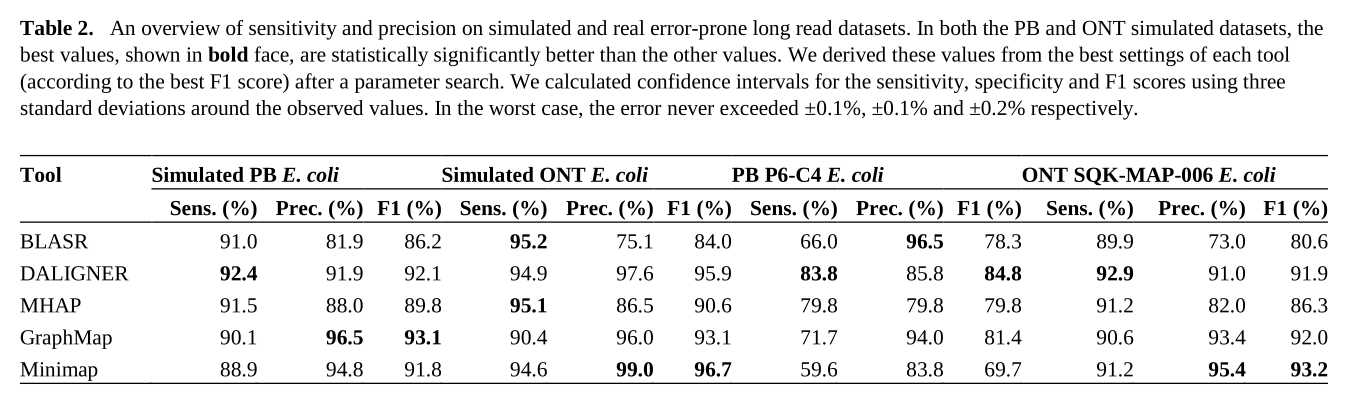
\includegraphics[width=\textwidth]{paper/blog_post/table_res_review.png}
\caption{Table 2 of \cite{ovl_bench}}
\end{figure}

Overlappers show better results on synthetic datasets than on real data.
We can observe an important loss of sensitivity: 59.6-83.8\% on the
Pacbio real dataset, compared to 88.9-92.4\% on the simulated data.

So, ok, overlappers dont't achieve perfect sensibility, but \textbf{do
they miss the same overlaps}?

\subsection{Materials \& Methods}\label{preassembly:ovl:materials-methods}

\subsubsection{Datasets}\label{preassembly:ovl:datasets}

I selected the two real sequencing datasets in \citeauthor{ovl_bench},
because they had the highest variance in sensitivity, so we can see the
most extreme effects in how long-read overlappers possibly find
different overlaps.

\subsubsection{What is an overlap}\label{preassembly:ovl:what-is-an-overlap}

I will not bore you with formal definitions :)

We will consider 3 type of overlaps, according to Algorithm 5 presented
in the minimap publication\cite{minimap} 

\begin{figure}[ht]
\centering
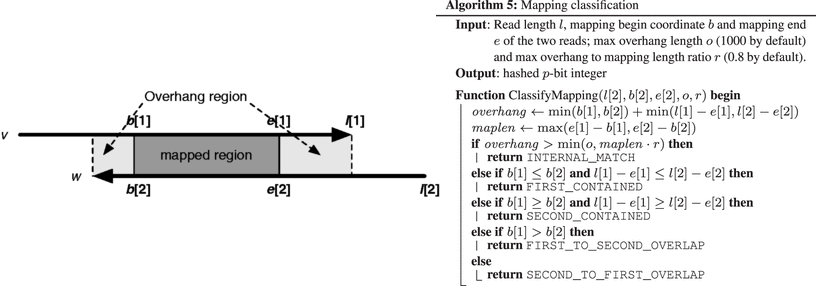
\includegraphics[width=\textwidth]{paper/blog_post/minimap_ovl_filter.png}
\caption{Algorithm 5 in minimap and miniasm article by Heng Li}
\end{figure}

\begin{description}
\item[Internal match:] Just a short similarity localized in the middle section of both reads,
which is probably due to a repetitive region and not a true overlap
\item[Containment:] One read is completely contained in another
\item[Classic overlap:] Deemed a regular suffix-prefix overlap
\end{description}

We will check the results of overlappers, and for each entry that isn't
an internal match nor an containment overlap, we store the pair of reads
as elements of the set of all overlaps found by the overlapper.

\subsubsection{Overlappers}\label{preassembly:ovl:overlappers}

We used:

\begin{itemize}
\item graphmap v0.5.2 \cite{graphmap}
\item hisea commit: 39e01e98ca \cite{hisea}
\item mhap 1.6 and 2.1 \cite{Berlin2015}
\item minimap 0.2-r124 \cite{minimap}
\item minimap2 2.10 \cite{minimap2}
\end{itemize}

We used parameters recommended by \citeauthor{ovl_bench} and default parameters for HISEA.

\subsubsection{Venn diagram generation}\label{preassembly:ovl:venn-diagram-generation}

We used a Python script to parse the output file of each overlapper,
filter overlaps, generate a Venn diagram, and compute the Jaccard index.
All scripts and steps to reproduce this analysis are available in this
\href{https://github.com/natir/SOTA-long-read-overlapping-tools-comparative-analysis-data}{repository}.

\subsection{Results}\label{preassembly:ovl:results}

\subsubsection{Nanopore real data}\label{preassembly:ovl:nanopore-real-data}

\begin{figure}[ht]
\centering
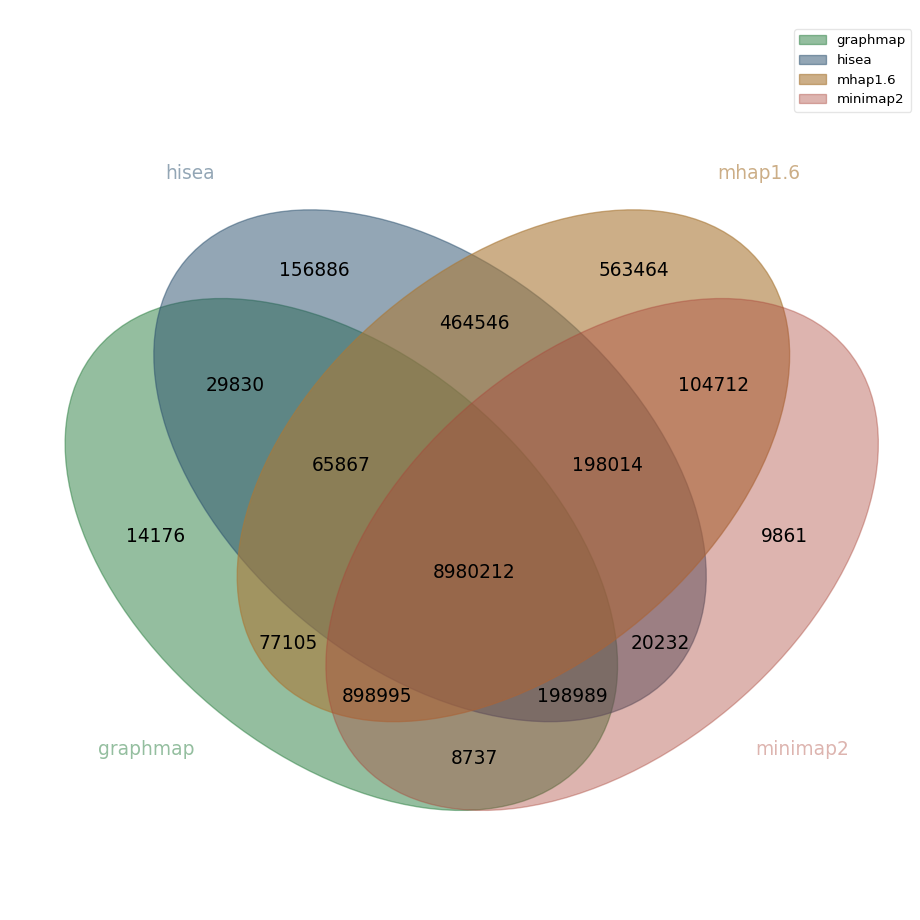
\includegraphics[width=0.4\textwidth]{paper/blog_post/nanopore_venn.png}
\caption{Venn diagram for nanopore real dataset}
\end{figure}

In the center of the above diagram we have the number of overlaps found
by all overlappers. We call this set the \emph{core overlaps}. Here for
this dataset, core overlaps contain 8,980,212 overlaps. Around this
center, we highlight some of the largest disparities between
overlappers:

\begin{table}[ht]
\centering
\begin{tabular}{lrr}
\hline
dataset composition & number of overlaps & \% of core overlaps \\
\hline
core overlaps - hisea overlaps & 898,995 & 10.01 \% \\
hisea overlaps \(\cap\) mhap overlaps & 464,546 & 5.17 \% \\
core overlaps - mhap overlaps & 198,989 & 2.21 \% \\
core overlaps - graphmap overlaps & 198,014 & 2.21 \% \\
\hline
\end{tabular}
\end{table}

In addition, out of the 11,352,915 overlaps found by mhap, 4.96 \% of
these are found only by this overlapper. For hisea, the corresponding
value is 1.55 \% (out of 10,114,576 overlaps).

\begin{table}[ht]
\centering
\begin{tabular}{rrrrr}
\hline
& mhap & minimap2 & graphmap & hisea \\
\hline
mhap & & 0.88 & 0.85 & 0.82 \\
minimap2 & 0.88 & & 0.94 & 0.84 \\
graphmap & 0.85 & 0.94 & & 0.83 \\
hisea & 0.82 & 0.84 & 0.83 & \\
\hline
\end{tabular}
\end{table}
The above matrix shows the Jaccard similarity coefficient (cardinality
of intersection divided by cardinality of union) between pairs of
overlappers.

\subsubsection{Pacbio real data}\label{preassembly:ovl:pacbio-real-data}

\begin{figure}[ht]
\centering
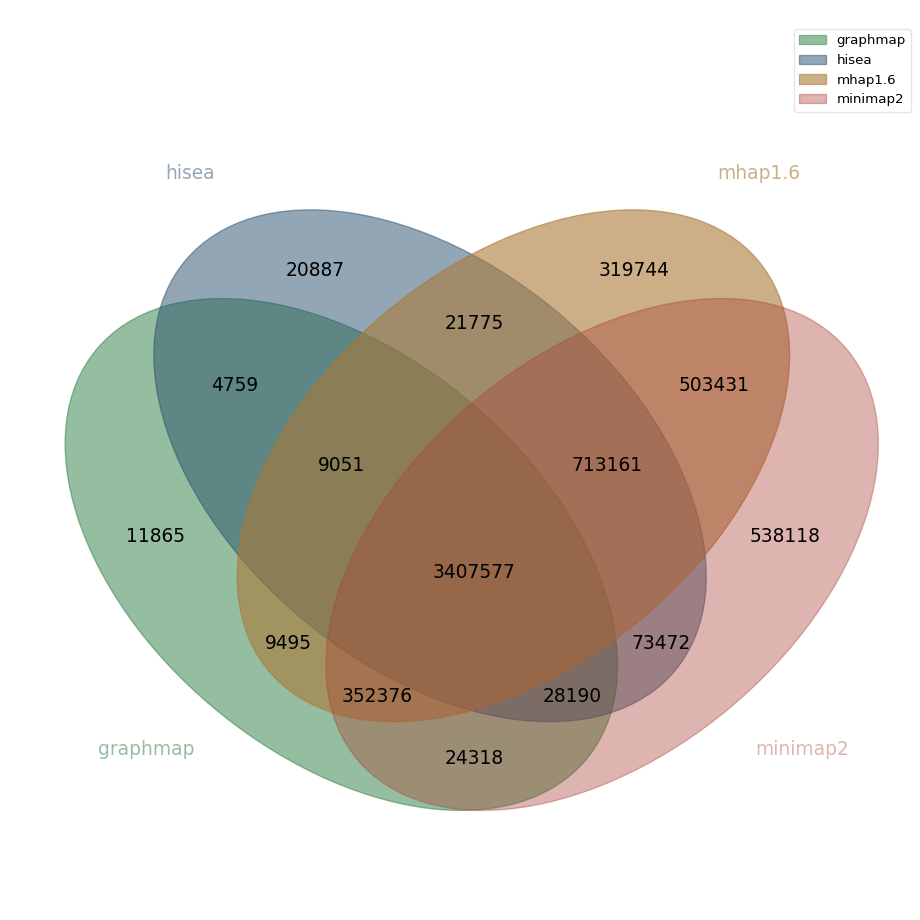
\includegraphics[width=0.4\textwidth]{paper/blog_post/pacbio_venn.png}
\caption{Venn diagram for pacbio real dataset}
\end{figure}

For the Pacbio dataset, core overlaps contain 3,407,577 overlaps. Other
large disparities between overlappers are:

\begin{table}[ht]
\centering
\begin{tabular}{lrr}
\hline
dataset composition & number of overlaps & \% of core overlaps \\
\hline
core overlaps - graphmap overlaps & 713,161 & 20.93 \% \\
minimap2-only overlaps & 538,118 & 15.79 \% \\
mhap overlaps \(\cap\) minimap2 overlaps & 503,431 & 14.77 \% \\
core overlaps - hisea overlaps & 352,376 & 10.44 \% \\
mhap-only overlaps & 319,744 & 9.38 \% \\
\hline
\end{tabular}
\end{table}

Out of all overlaps found by minimap2 (5,640,643), 9.54\% of these
overlaps are found only by this overlapper, for mhap the corresponding
value is 5.98\% (out of 5,336,610 overlaps).

\begin{table}[ht]
\centering
\begin{tabular}{rrrrr}
\hline
& mhap & minimap2 & graphmap & hisea \\
\hline
mhap & & 0.83 & 0.70 & 0.76 \\
minimap2 & 0.83 & & 0.67 & 0.74 \\
graphmap & 0.70 & 0.67 & & 0.74 \\
hisea & 0.76 & 0.74 & 0.74 & \\
\hline
\end{tabular}
\end{table}

Again the above matrix shows Jaccard similarity coefficient.


\subsubsection{Comparison across versions}\label{preassembly:ovl:comparison-across-versions}

At first we used mhap 2.1, using the same parameters as in \citeauthor{ovl_bench}
But actually, \citeauthor{ovl_bench} used mhap 1.6. This version change
yielded surprising results: many more overlaps were found only by mhap
2.1. Here is a comparison between the two executions of mhap 1.6 and 2.1
using the same command-line parameters, in terms of shared and exclusive
overlaps.

\begin{figure}[ht]
\centering
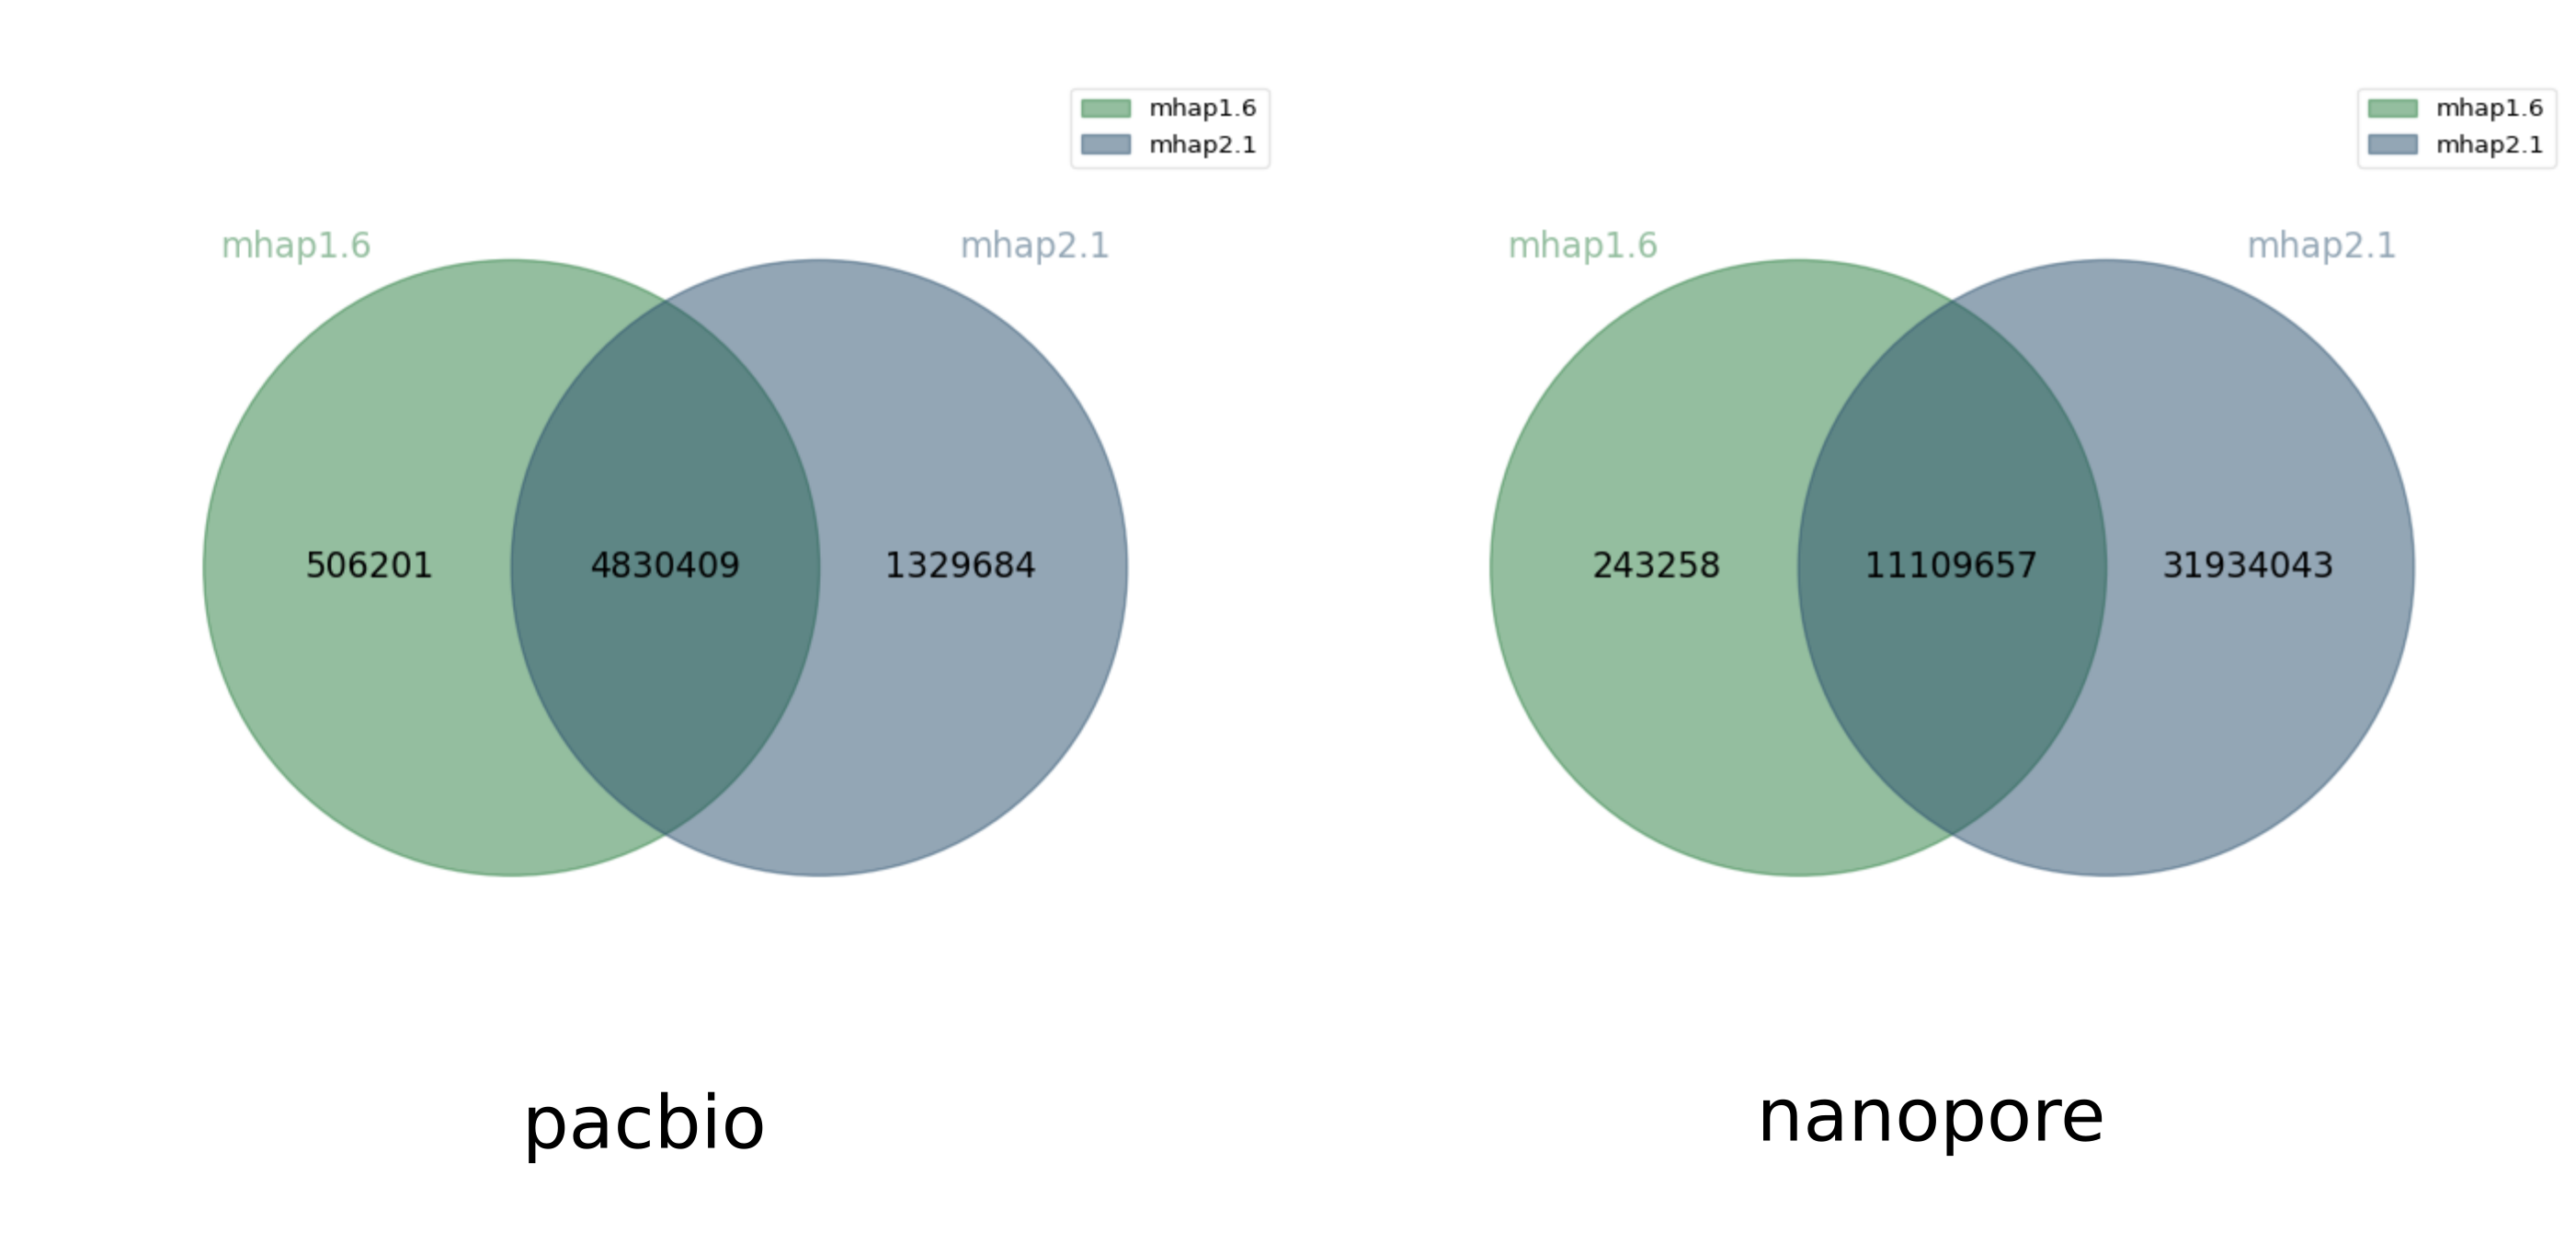
\includegraphics[width=0.7\textwidth]{paper/blog_post/mhap_venn_same.png}
\caption{Jaccard similarity 0.72, 0.26}
\end{figure}



mhap 2.1 found many more overlaps than mhap 1.6. But it turns out that
this is because mhap 1.6 calculates a similarity score between reads and
mhap 2.1 calculates a distance between reads, the meaning of the
-\/-threshold option is different between the two versions, so we should
have not used the same parameter value for both versions (thanks to
Sergey Koren for pointing this out). This explains why a user may get
significantly different results between the two versions, when running
them carelessly with identical parameters. Below, we plot the Venn
diagrams of overlaps found only by mhap 1.6 with -\/-threshold 0.02 for
pacbio and -\/-threshold 0.04 (like Chu. \emph{et al}) and only by mhap
2.1 with -\/-threshold 0.75 for pacbio and -\/-threshold 0.78 for
nanopore.

\begin{figure}[ht]
\centering
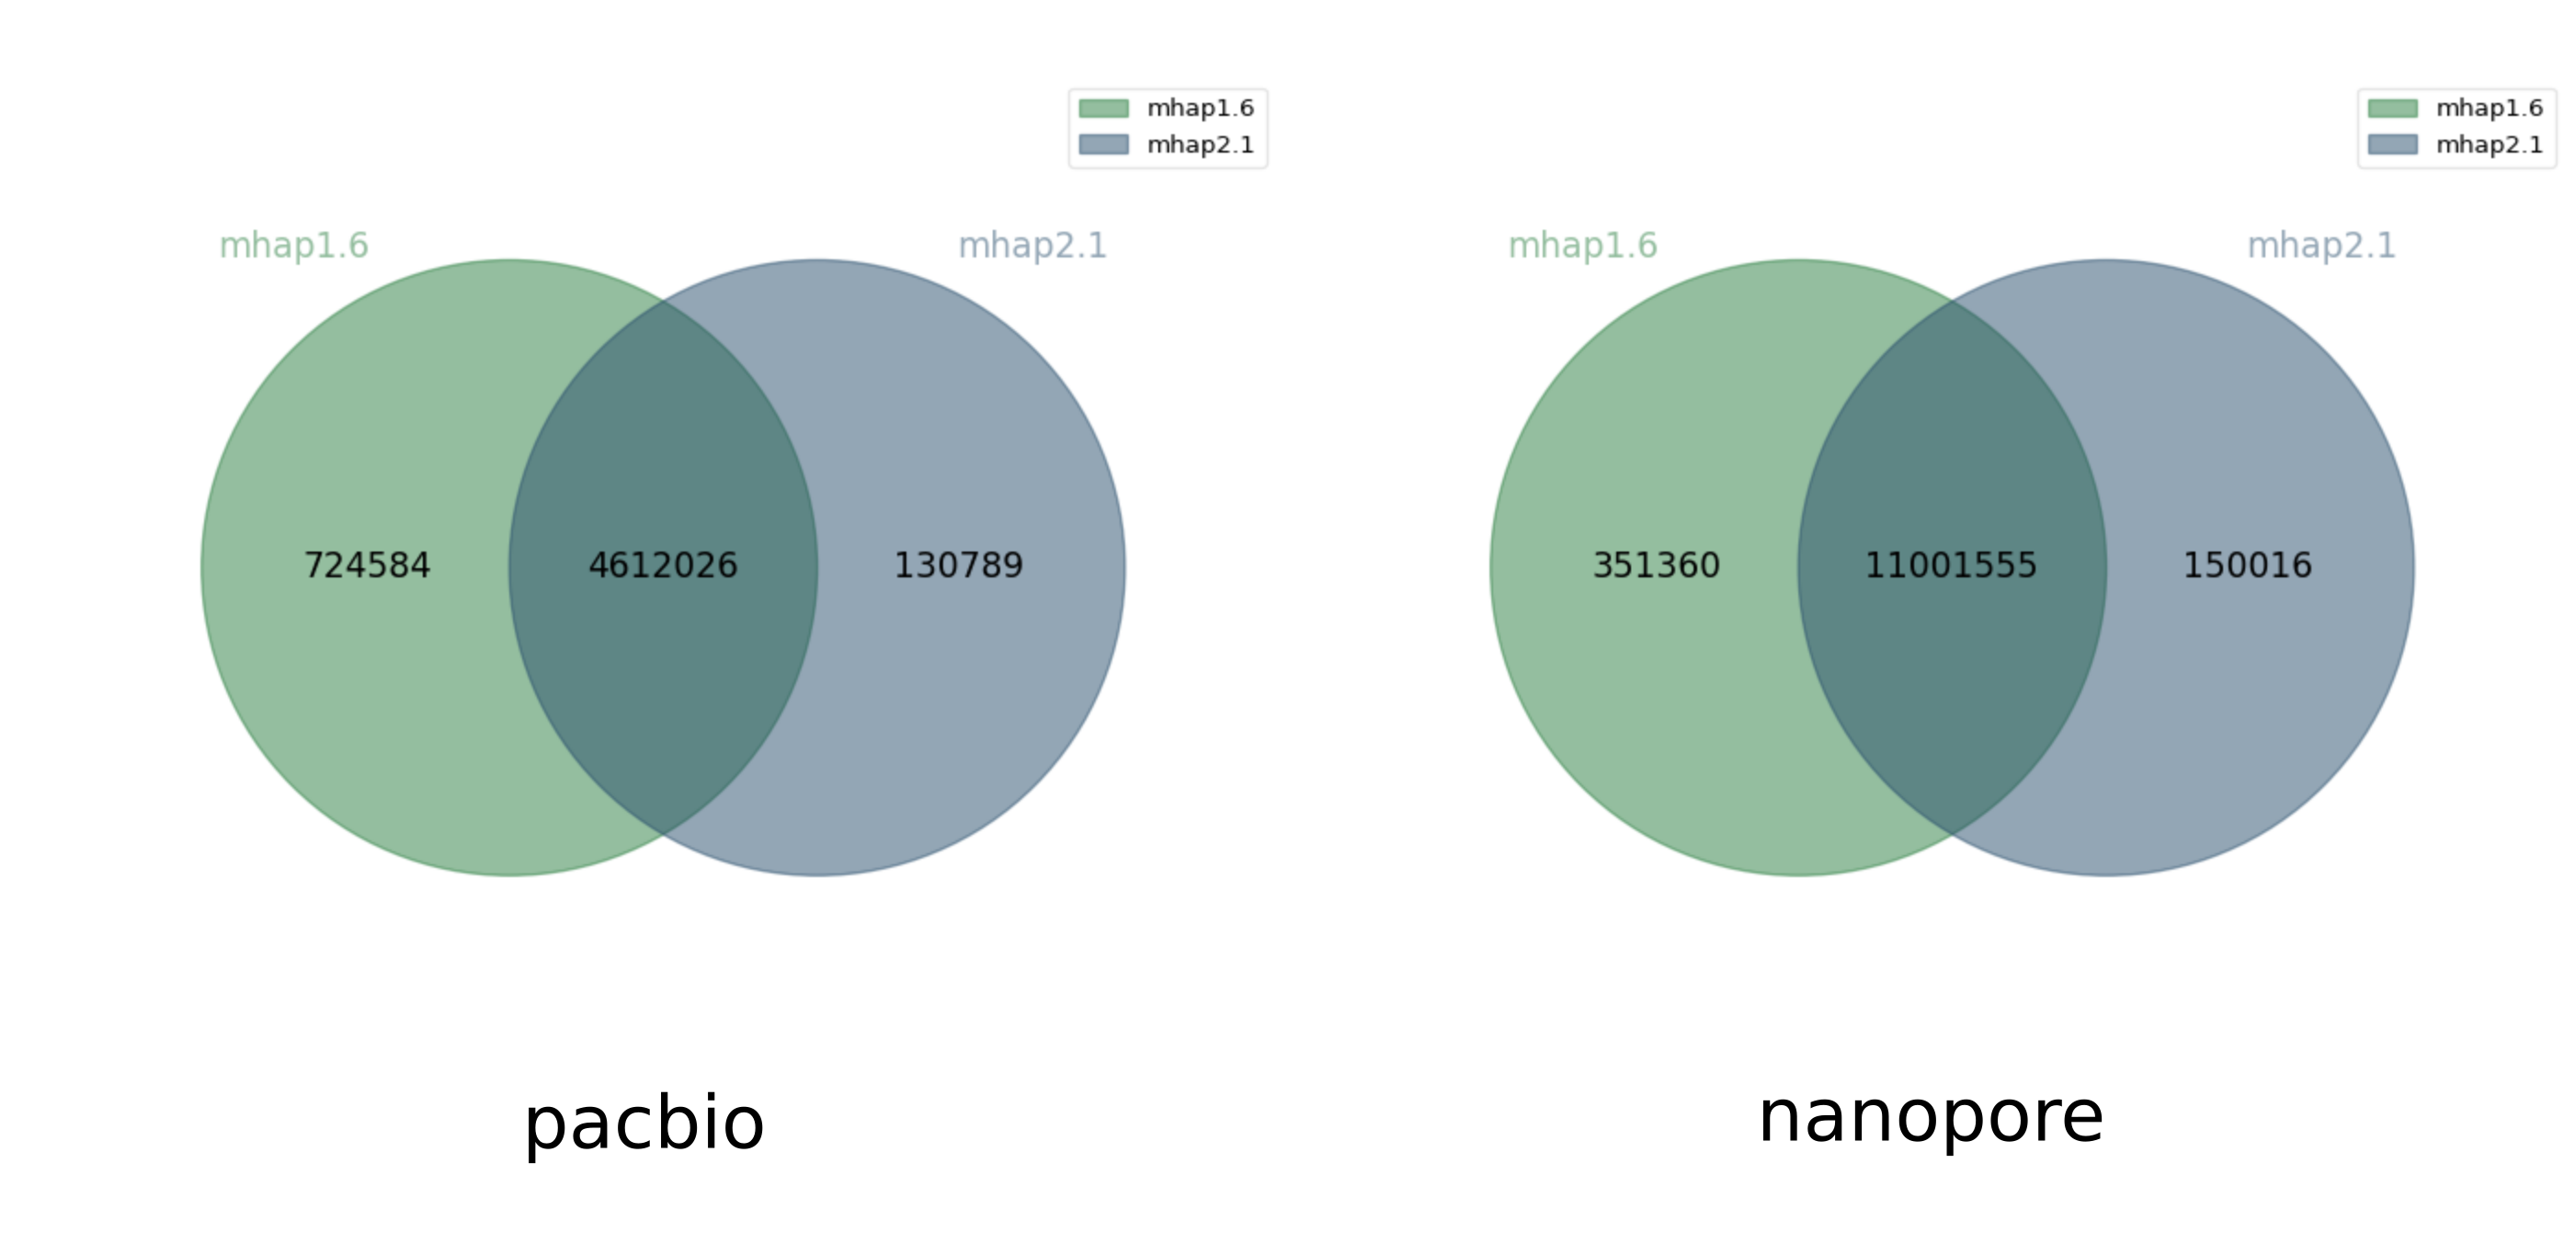
\includegraphics[width=0.7\textwidth]{paper/blog_post/mhap_venn.png}
\caption{Jaccard similarity 0.84, 0.96}
\end{figure}


Both software find roughly the same set of overlaps, with the trend that
mhap1.6 tended to find a bit more (it would be interesting to evaluate
whether those were correct or wrong overlaps).

And another comparison between minimap and minimap2:

\begin{figure}[ht]
\centering
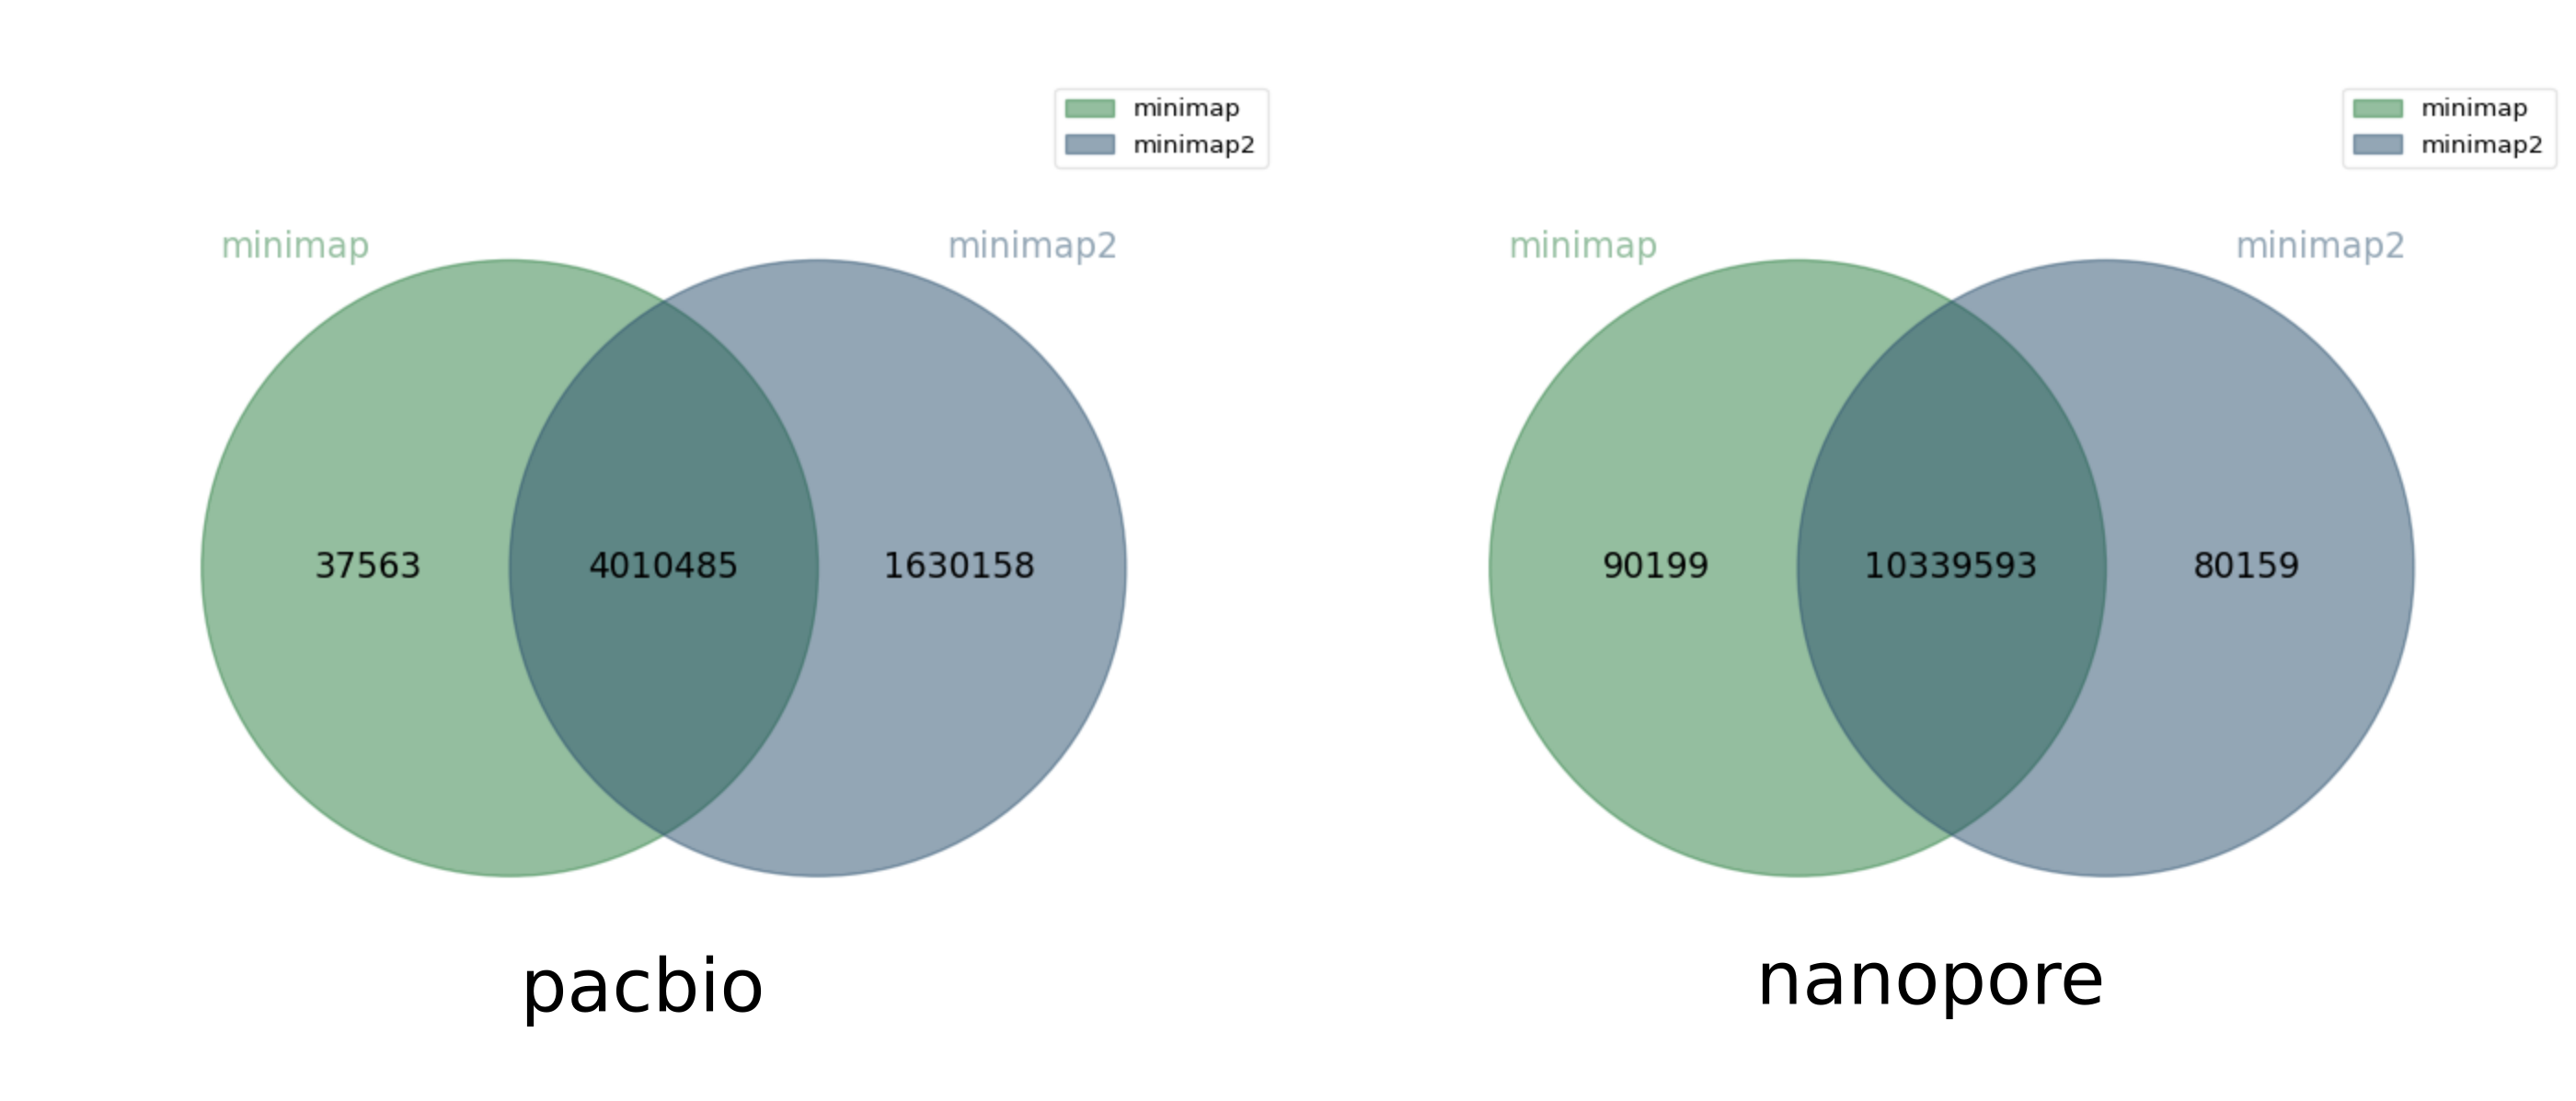
\includegraphics[width=0.7\textwidth]{paper/blog_post/minimap_venn.png}
\caption{Jaccard similarity 0.71, 0.98}
\end{figure}


For the pacbio dataset, minimap2 finds significantly (1.6M) more
overlaps than minimap (which found 4M overlaps). But for the nanopore
dataset, both software roughly agree.

\subsection{Conclusion}\label{preassembly:ovl:conclusion}

Overlapper tools behave quite similarly, but on real pacbio
datasets sensibility, precision, and the set of overlaps found across tools can
be very different. Such a difference can also exist between two versions
of the same tool.

Comparison of overlappers based on a quantitative measurement
(sensitivity, precision) is useful but isn't perfect: two tools with the
same sensitivity for a given set could still detect a different set of
overlaps, see e.g.~mhap and minimap2 for the nanopore set.

Some publications use quality of error-correction, or results of genome
assembly, as quality metrics to compare overlappers. It's a good idea
but correction and assembly tools make additional choices in the
overlaps they keep, and it's not easy to relate assembly or
error-correction imperfections and wrong or missed overlaps.

From our tests, there is no clear best overlapper software so far.

It could by interesting to study whether certain tools have a bias when
finding overlaps, linked to e.g length of reads, mapping length, error
rate, \%GC, specific kmer composition, etc \ldots{} A study like this
could possibly reveal some intrinsic properties of the algorithms used
in overlappers.

Is it a good idea to create a reconciliation tool for overlappers? We
note that the correction and assembly tools seek to reduce the amount of
overlaps they use, through e.g.~graph transitivity reduction, Best
Overlap Graph, the MARVEL approach (Supplementary information of \cite{MARVEL}).

\subparagraph{Acknowledgment}\label{preassembly:ovl:acknowledgment}

\begin{itemize}
\item Sergey Koren
\item Rayan Chikhi
\item Jean-Stéphane Varré
\end{itemize}

\end{document}